\section{Konklusjon og anbefalinger}
\label{sec:konklusjon}
\textit{Kort oppsummering av den innsikt som er oppnådd som er aktuelt for videreføring i Fase II. Enkelt-resultater som kan tallfestes bør være med.\\
\\
NB: Vær konkret på dette punktet. Det er uinteressant \textbf{at} gruppen har oppnådd innsikt på det ene eller andre området. Det interessante er \textbf{hvilken} innsikt som er oppnådd. \\
\\
Anbefalinger for videreføring, bruk og vedlikehold er også viktig å få med.}


\subsection{Videreutvikling}

\subsubsection{Mesh-nettverk}

Systemet vårt har slik det er nå en stor svakhet: vi detekterer bare aktivitet fra en side av turbinen. Med vårt system med et kamera, vil vi ha store mørketall siden vi bare detekterer fra en retning. Derfor vil det være lurt som en videreutvikling av systemet å utvide til en mesh-struktur bestående av flere noder med kamera og prosseseringsenhet. Dette kan løses ved at i tillegg til det enkelte systemet med værstasjon og kamera så er det plassert flere noder med for eksempel bare kameramodulen for å "se" et større område. En skisse er vist i figur \ref{fig:fraoven}.

\begin{figure}[H]
    \centering
    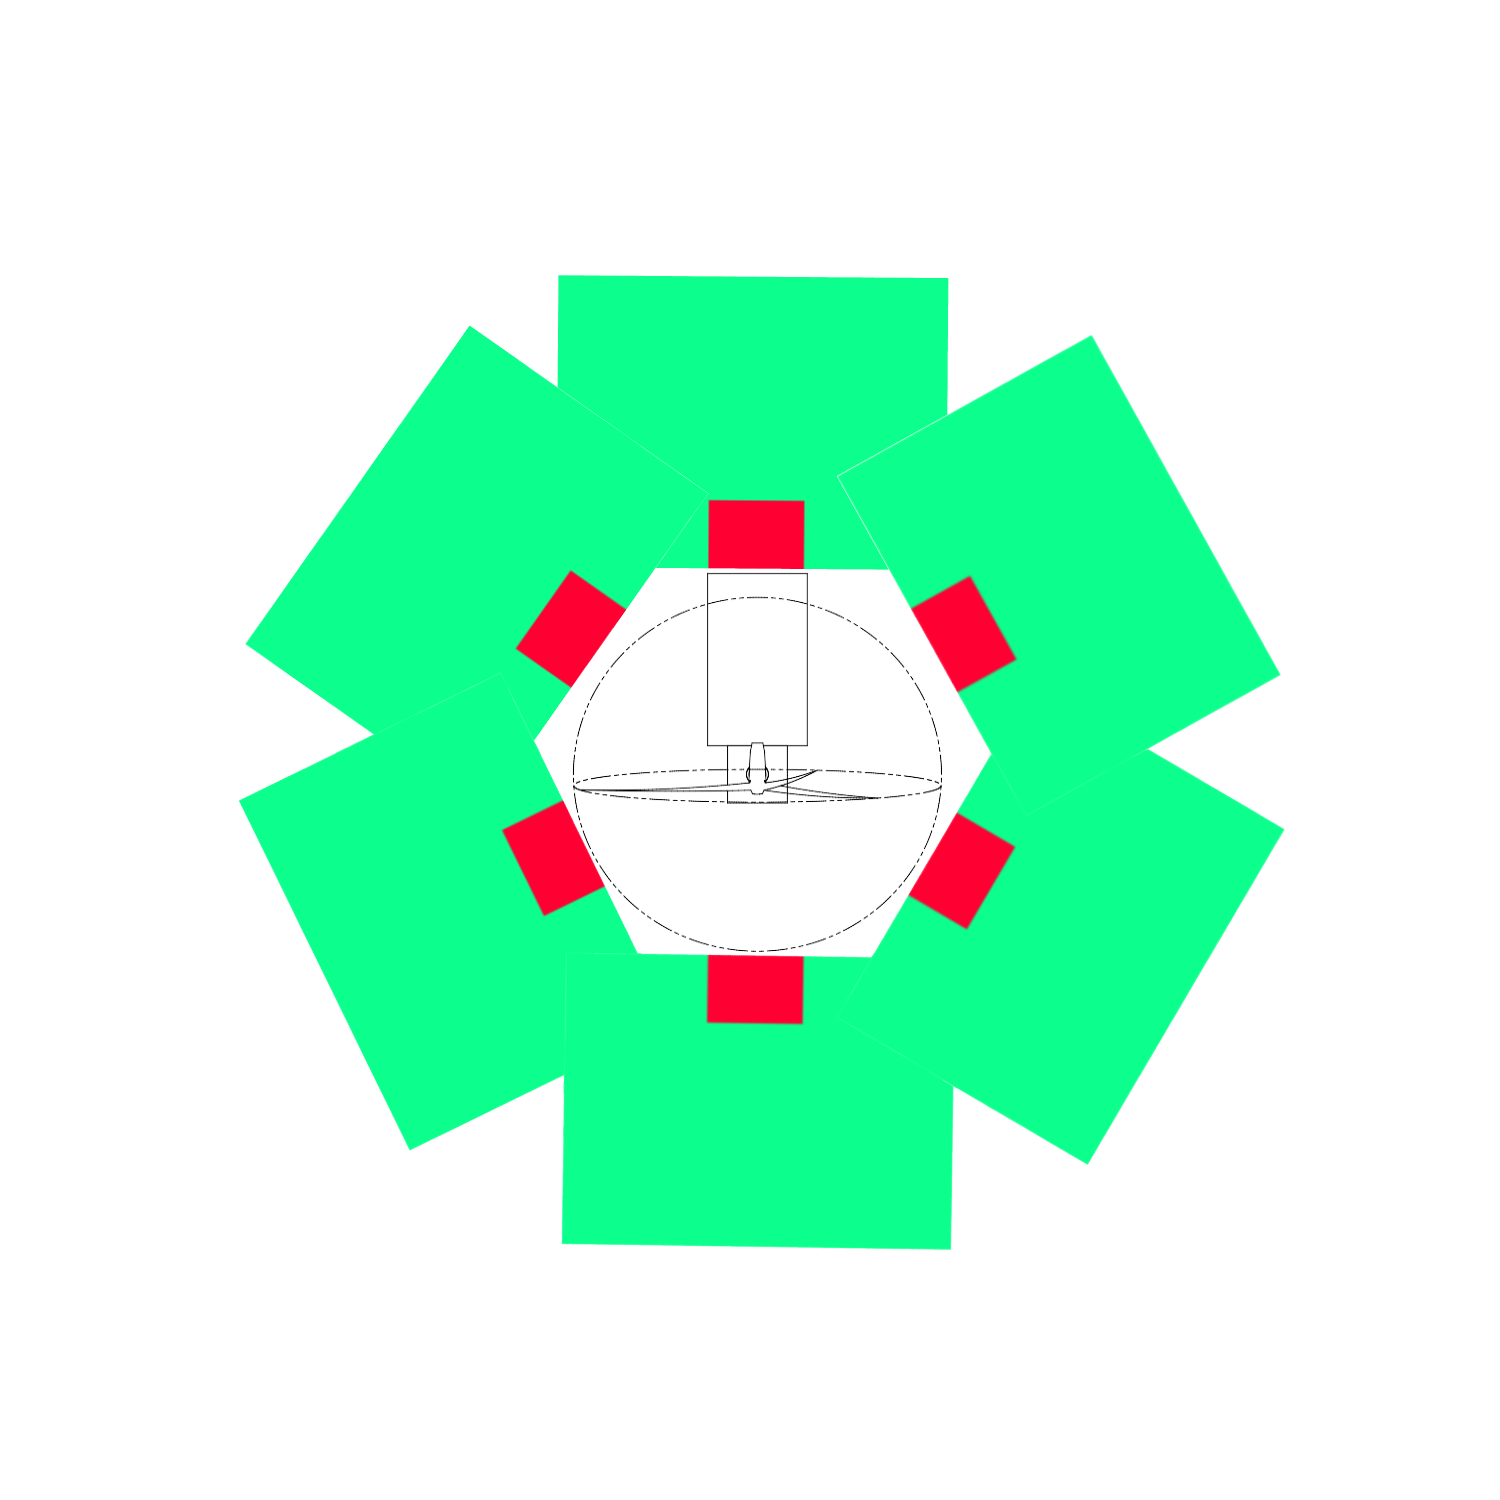
\includegraphics[width=0.7\textwidth]{konklusjon/Nettverk.png}
    \caption{Konsept på hvordan fire kameraer kan detektere fugletrafikk inn mot en vindturbin fra alle retninger. I grønt er deteksjonsområdet, rødt er boksenes plassering.}
    \label{fig:fraoven}
\end{figure}


Dette kan også hjelpe i områder uten vindkraftutbygging der man skal telle fugler på et større område. Dette vil gi en høyere sikkerhet i telte fugler, der en fugl som ikke blir telt av et kamera kan bli telt av et annet. Dette vil også lettere kunne fastslå fuglenes adferd og potensielt finne fram til den ideelle vindturbinplasseringen for minst mulig påvirkning på fuglelivet. 

En vil også potensielt kunne koble flere kameraer til en sentral prossesseringsenhet som "syr sammen" videoen fra kameraene og gir et mer helhetlig bilde av fugleaktiviteten. Systemet vil da kunne klare å følge en fugl og dens aktivitet over større områder. Dette bil også gjøre systemet mer beskyttet for svikt i kameraene, da om et kamera svikter så vil resten fortsatt klare å telle fugler. 

Det er to grunner til at dette ikke har blitt gjennomført: penger og tid. Kamera er den dyreste komponenten vi jobber med, der prisen for et kamera er på 700\$. Når dette prosjektet også foregår over et semester ser vi ikke nødvendigheten i å bruke tid på å potensielt gjøre samme arbeid flere ganger, ved å sette opp enda en kameraboks. 

\subsubsection{Synsvidde}
Om kameraet ikke ser nok foran vindturbinen vil det kunne være mulig å oppgradere kameraet til et med større synsfelt. Dette vil gi oss større område per kamera å detektere fugler og kan gi oss bedre data på å forutsi banen fuglen vil ta, da vi har flere potensielle målinger. Om oppløsningen forblir den samme vil vi potensielt få færre piksler å jobbe med, som vi gi mindre nøyaktighet, men større område. Om oppløsningen blir skalert vil vi få lik nøyaktighet, men et større målingområde, som fører til større bilder i størrelse og da mer potensielt mer prosessering per bilde.

\subsubsection{Trådløs}
For at produktet skal virke optimalt før vindturbiner er satt opp så vil dette kreve at systemet ikke bruker nettstrøm. \todo{finne wattage med dagens løsning.}

\subsection{Bruk}



\subsection{Konklusjon}

\subsection{Takk}

Takk til institutt for elkraftteknikk for lån av Flir C3.
